\section{Obbiettivo}

RIEMPIMI

\section{Ambiente di Lavoro}

Questa esercitazione \`{e} stata svolta all'interno del seguente ambiente di lavoro:

\begin{itemize}
	\item \textbf{Hardware}: 
		\begin{itemize}
			\item \textbf{CPU}: AMD Ryzen 9 5900x
			\item \textbf{RAM}: 32 GB DDR4 @3200 MHz
		\end{itemize}
	\item \textbf{Software}:
		\begin{itemize}
			\item \textbf{Host OS:} Arch Linux
			\item \textbf{Guest OS}: Ubuntu 20.4 LTS Server
			\item \textbf{Virtualization Software}: VirtualBox 6.1
		\end{itemize}
\end{itemize}

\section{Configurazione Macchine}

Per questa esercitazione sono necessarie 3 macchine virtuali che saranno 1 \lstinline[style=cmd]|master|, il quale avr\`{a} il compito di accettare i job e di effettuare lo scheduling di questi e 2 \lstinline[style=cmd]|slave| che avranno il compito di eseguire i vari job assegnategli . Ogni macchina \`{e} stata configurata come segue:

\begin{itemize}
	\item \textbf{Cores:} 4 Core
	\item \textbf{RAM:} 4 GB
	\item \textbf{Dischi di archiviazione:}
		\begin{itemize}
			\item Disco Principale da 10 GB
		\end{itemize}
	\item \textbf{Scheda di Rete:} Scheda di rete con Bridge
\end{itemize}
\ \\
\`{E} consigliato configurare una sola macchina, installare e configurare il sistema operativo e i software necessari, per poi utilizzare la funzione 'Clona' di VirtualBox per generare una copia identica senza dover ripetere tali operazioni nuovamente. Durante la fase di clonazione della macchina \`{e} necessario selezionare l'opzione "Generare nuovi Mac Address per ogni Network Adapter" come policy per la gestione dei Mac Address.

\begin{center}
	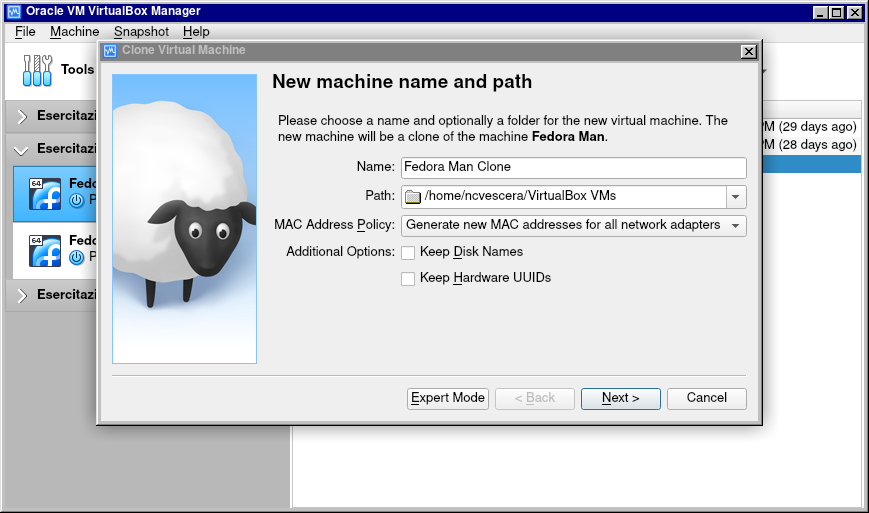
\includegraphics[width=\textwidth]{screens/vb_macpolicy.png}
\end{center}

\section{Configurazione Software}

\subsection{Sistema Operativo}

Appena terminata la configurazione della macchina virtuale aggiungo la iso di Ubuntu 20.4 Server e avvio la fase di installazione.\\
Seleziono la lingua del sistema e il layout della tastiera:

\begin{center}
	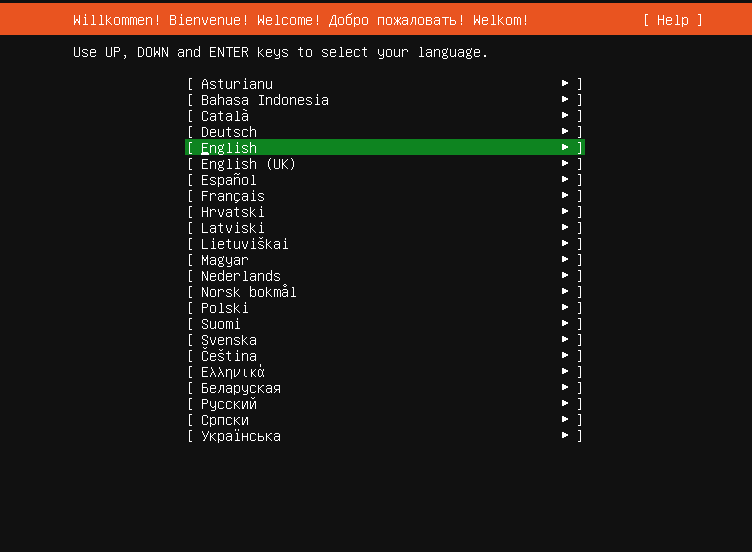
\includegraphics[width=0.6\textwidth]{screens/ubuntu_1.png}
\end{center}
\ \\
Mi assicuro che alla scheda di rete venga assegnato un IP dal DHCP per poter scaricare il software necessario durante l'installazione:

\begin{center}
	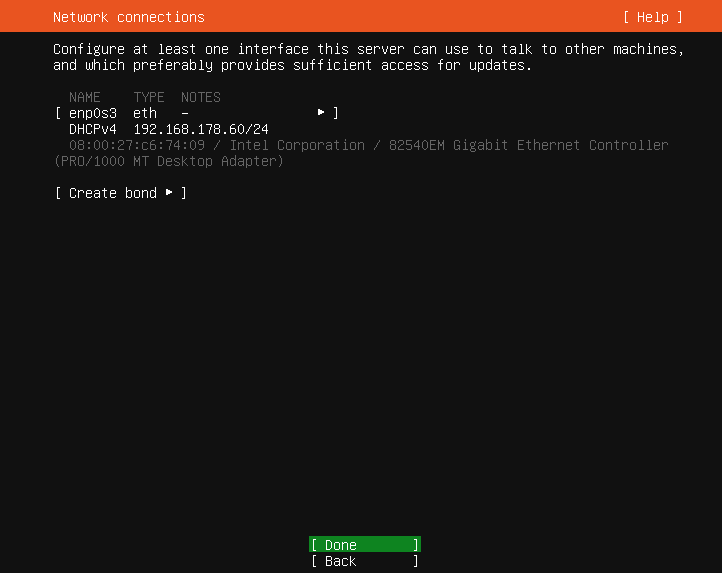
\includegraphics[width=0.6\textwidth]{screens/ubuntu_2.png}
\end{center}
\ \\
Ignoro la sezione del proxy e scelgo il mirror italiano:

	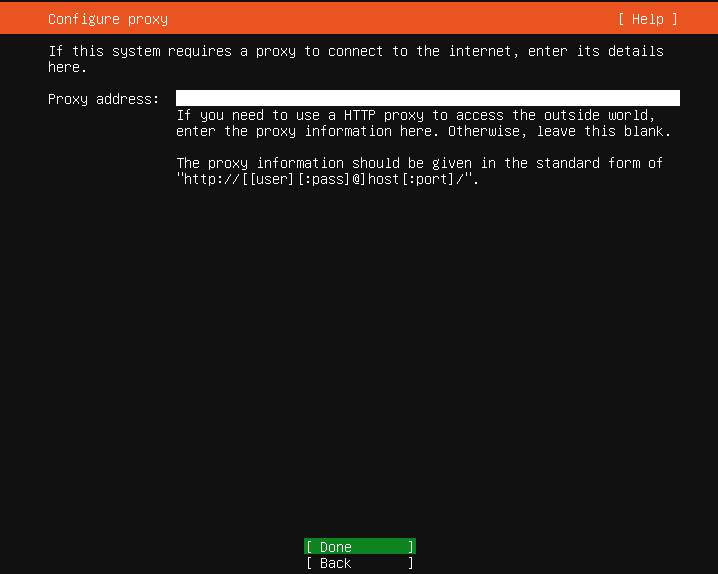
\includegraphics[width=0.5\textwidth]{screens/ubuntu_3.png}
	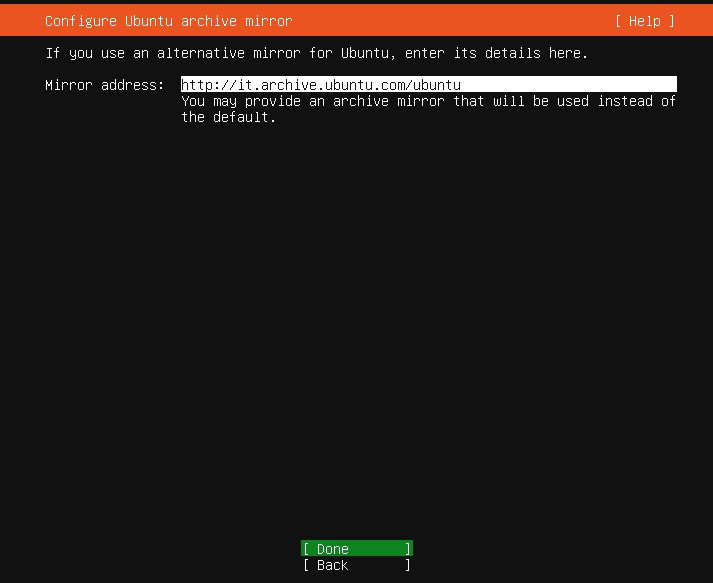
\includegraphics[width=0.5\textwidth]{screens/ubuntu_4.png}
\ \\
Formatto l'intero disco con le impostazioni consigliate:

	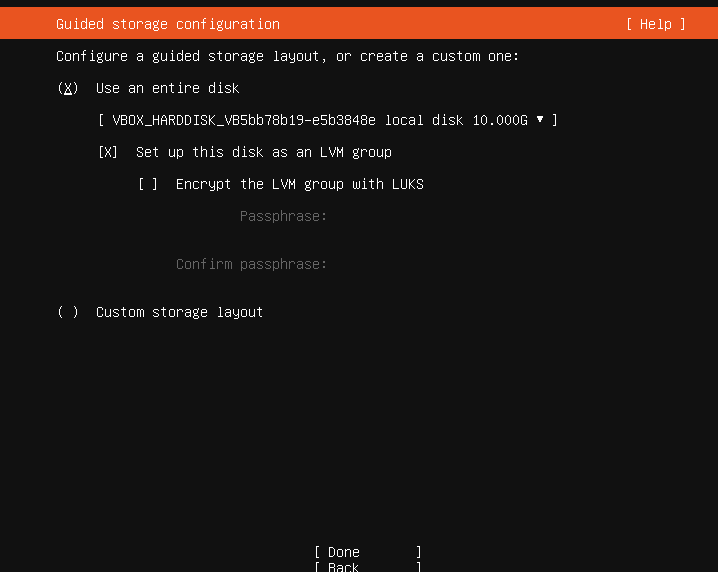
\includegraphics[width=0.5\textwidth]{screens/ubuntu_5.png}
	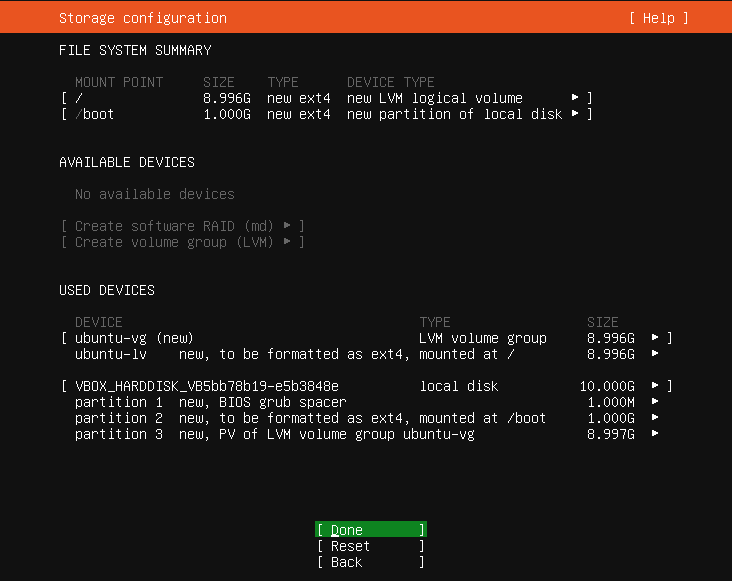
\includegraphics[width=0.5\textwidth]{screens/ubuntu_6.png}
\ \\
Creo un nuovo utente e scelgo la pasword:
\begin{center}
	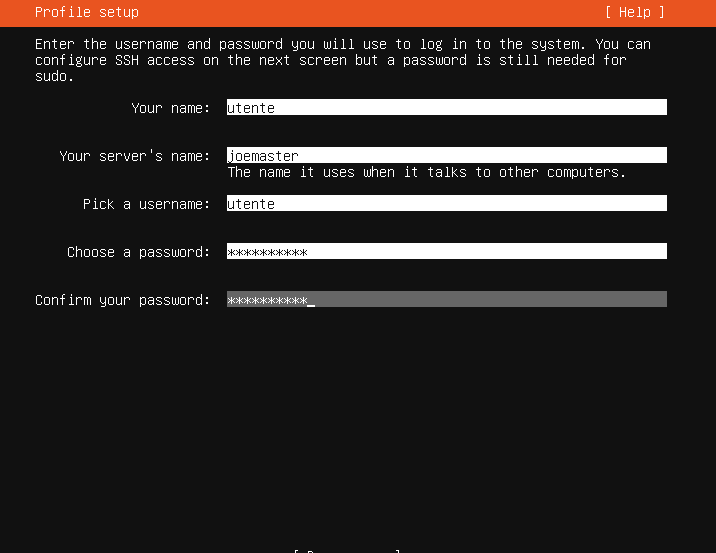
\includegraphics[width=0.6\textwidth]{screens/ubuntu_7.png}
\end{center}
\ \\
Mi assicuro che il servizio \icode{sshd} venga installato e abilitato;
\begin{center}
	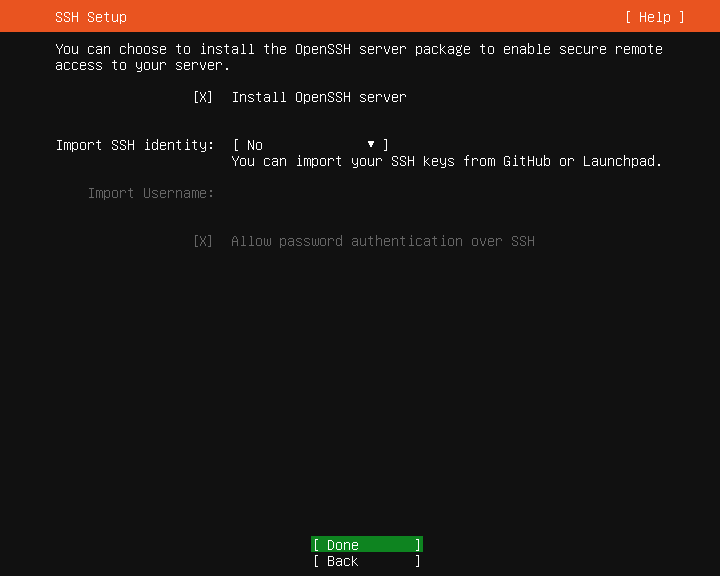
\includegraphics[width=0.6\textwidth]{screens/ubuntu_8.png}
\end{center}
\ \\
Completo l'installazione e riavvio la macchina:

\begin{center}
	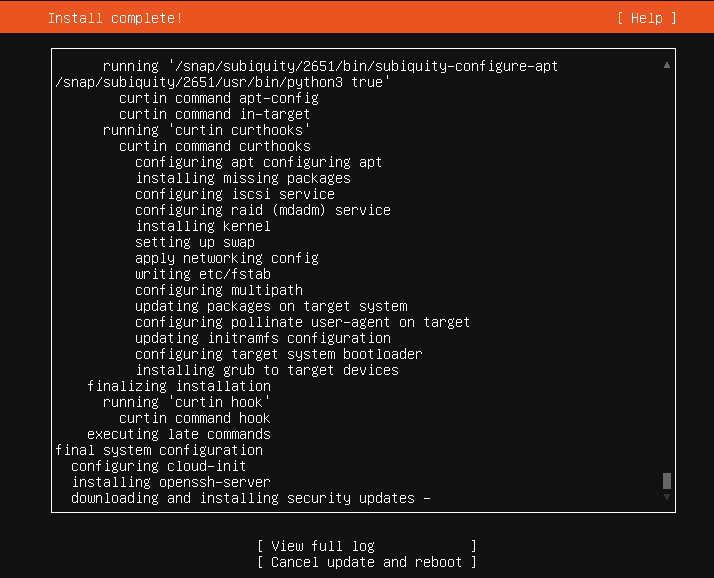
\includegraphics[width=0.6\textwidth]{screens/ubuntu_9.png}
\end{center}
	
\subsection{Software Necessario}

Appena ho terminato la fase di installazione del SO, ho provveduto ad aggiornarlo con i
seguenti comandi, per evitare problemi di compatibilit\`{a} e software obsoleto:

\begin{lstlisting}[style=cmd]
 sudo apt update
 sudo apt upgrade
\end{lstlisting}
\ \\
Poi ho installato i pacchetti necessari (\lstinline[style=cmd]|HTCondor| e \lstinline[style=cmd]|stress-ng|) con:

\begin{lstlisting}[style=cmd]
 sudo apt install htcondor 
 sudo apt install stress-ng
\end{lstlisting}
\ \\
Durante l'installazione del software \lstinline[style=cmd]|HTCondor| verr\`{a} mostrato un menu dove viene chiesto se utilizzare una configurazione gi\`{a} pronta di Condor, io ho scelto \lstinline[style=cmd]|No| in quanto ho preferito configurare tutto a mano per comprendere meglio il file di configurazione ed i vari parametri da modificare.\\
\ \\
Il pacchetto \lstinline[style=cmd]|stress-ng| serve per mettere sotto sforzo i vari core della macchina e verr\`{a} utilizzato in seguito per testare la configurazione dei due slave.

\subsection{IP}

Ho assegnato IP statici alle macchine per essere sicuro di poterle sempre raggiungere e che
il DHCP del mio router non gli assegni indirizzi diversi col passare del tempo.\\
Gli indirizzi che ho scelto sono:
\begin{itemize}
	\item Master: 192.168.178.57
	\item Slave 1: 192.168.178.54
	\item Slave 2: 192.168.178.59
\end{itemize}
Per farlo ho utilizzato la seguente procedura (\`{e} uguale per tutte le macchine, basta solo cambiare l'ip):

\begin{enumerate}
	\item Ho creato il file \lstinline[style=cmd]|99-disable-network-config.cfg| e l'ho popolato con la seguente configurazione:
	
	\begin{lstlisting}[style=cmd]
 echo "network: {config: disabled}" | sudo tee /etc/cloud/cloud.cfg.d/99-disable-network-config.cfg
	\end{lstlisting}
	\item Ho riscritto il file di configurazione \lstinline[style=cmd]|/etc/netplan/00-installer-config.yaml| con:
	
	\begin{lstlisting}[style=cmd]
 network:
   version: 2
   renderer: networkd
   ethernets:
     enp0s3:
       dhcp4: no
       addresses:
         - 192.168.178.57/24
       gateway4: 192.168.178.1
       nameservers:
         addresses: [8.8.8.8, 1.1.1.1]
	\end{lstlisting}
	\item Ho riavviato la macchina per rendere effettive le modifiche.
\end{enumerate}
\ \\
Per le altre macchine va modificato il parametro \lstinline[style=cmd]|addresses| con il corretto IP.\\
\ \\
Per controllare il corretto funzionamento di questa operazione basta utilizzare il comando \lstinline[style=cmd]|ifconfig enp0s3| e controllare che abbia il giusto indirizzo:

\begin{lstlisting}[style=output]
 enp0s3: flags=4163<UP,BROADCAST,RUNNING,MULTICAST>  mtu 1500
 inet 192.168.178.57  netmask 255.255.255.0  broadcast 192.168.178.255
 ...
\end{lstlisting}
 
 \subsection{hosts \& hostname}
 \label{sec:hosts}
 
 Ho modificato il file \lstinline[style=cmd]|/etc/hostname| definendo un nome diverso per ogni macchina in modo
 tale da poterle distinguere pi\`{u} facilmente durante le sessioni SSH:
 
 \begin{itemize}
 	\item Nome Macchina 1 (Master): \lstinline[style=cmd]|joemaster|
 	\item Nome Macchina 2 (Slave1): \lstinline[style=cmd]|joeslave1|
 	\item Nome Macchina 3 (Slave2): \lstinline[style=cmd]|joeslave2|
 \end{itemize} 
\ \\
In tutte le macchine, alla fine del file \lstinline[style=cmd]|/etc/hosts| ho aggiunto le seguenti righe per
facilitare poi la configurazione di htcondor:

\begin{lstlisting}[style=cmd]
 192.168.178.57	nodo1	nodo1.condor
 192.168.178.54	nodo2	nodo2.condor
 192.168.178.59	nodo3	nodo3.condor
\end{lstlisting}

\subsection{Firewall}

Per evitare problemi di comunicazione tra le varie macchine ho deciso di disabilitare il firewall.\\
In Ubuntu 20.4 LTS solitamente il firewall \`{e} disabilitato. Ho comunque controllato con il comando:

\begin{lstlisting}[style=cmd]
 sudo ufw status
\end{lstlisting}
\ \\
Se ho questo output vuol dire che il servizio non \`{e} attivo:

\begin{lstlisting}[style=output]
 Status: inactive
\end{lstlisting}
\ \\
In caso contrario lo andr\`{o} a disabilitare con:

\begin{lstlisting}[style=cmd]
 sudo ufw disable
\end{lstlisting}

\subsection{Configurazione HTCondor}

In ogni macchina ho modificato il file di configurazione di HTCondor \lstinline[style=cmd]|/etc/condor/config.d/00personal_condor.config| in modo opportuno in base al compito che dovr\`{a} svolgere. Di seguito ho riportato le varie configurazioni per il Master e gli Slave.


\subsubsection{JoeMaster}

\begin{lstlisting}[style=cmd]
 CONDOR_HOST = nodo1
 COLLECTOR_NAME = Personal Condor at $(FULL_HOSTNAME)
 
 START = TRUE
 SUSPEND = FALSE
 CONTINUE = TRUE
 KILL = FALSE
 
 DAEMON_LIST = COLLECTOR, MASTER, NEGOTIATOR, SCHEDD
 
 HOSTALLOW_WRITE = *.condor
\end{lstlisting}
\ \\
Nella lista \lstinline[style=cmd]|DAEMON_LIST| manca \lstinline[style=cmd]|STARTD| in quanto il master non deve eseguire job, ma solo riceverli ed assegnarli ai vari slave.\\
\ \\
La variabile \lstinline[style=cmd]|CONDOR_HOST| indica qual \`{e} il nodo master, nel mio caso \lstinline[style=cmd]|node1| per via della configurazione in \autoref{sec:hosts}. Questo sar\`{a} uguale anche per gli Slave.\\
\ \\
Con \lstinline[style=cmd]|HOSTALLOW_WRITE| vado ad autorizzare tutti gli host all'interno del dominio \lstinline[style=cmd]|condor|, definito in \autoref{sec:hosts}.
	
\subsubsection{JoeSlave1/JoeSlave2}
\label{sec:joeslave}

\begin{lstlisting}[style=cmd]
 #Macro(n)
 NonCondorLoadAvg = (LoadAvg - CondorLoadAvg)
 HighLoad = 0.6
 BgndLoad = 0.3
 CPU_Busy = ($(NonCondorLoadAvg) >= $(HighLoad))
 CPU_Idle = ($(NonCondorLoadAvg) <= $(BgndLoad))
 KeyboardBusy = (KeyboardIdle < 10)
 MachineBusy = ($(CPU_Busy) || $(KeyboardBusy))
 ActivityTimer = (CurrentTime - EnteredCurrentActivity)
 
 CONDOR_HOST = nodo1
 COLLECTOR_NAME = Personal Condor at $(FULL_HOSTNAME)
 
 WANT_SUSPEND = True
 WANT_VACATE = True
 
 START =  $(CPU_Idle) && !$(KeyboardBusy)
 SUSPEND = $(MachineBusy)
 CONTINUE = $(CPU_Idle) && KeyboardIdle > 120
 PREEMPT = (Activity == "Suspended") && $(ActivityTimer) > 120     
 KILL = $(ActivityTimer) > 300

 DAEMON_LIST = MASTER, STARTD
 
 HOSTALLOW_WRITE = *.condor
\end{lstlisting}
\ \\
La configurazione per gli slave \`{e} la medesima in quanto avranno tutti e due lo stesso comportamento: dovranno interrompere l'esecuzione del job se viene registrata attivit\`{a} della tastiera (vengono considerate anche le sessioni remote come ssh) o se il carico della CPU supera una certa soglia.\\
Tramite le variabili \lstinline[style=cmd]|START, SUSPEND e WANT_SUSPEND| e le Macro \lstinline[style=cmd]|CPU_Idel, KeyboardBusy e MachineBusy| riesco ad ottenere il comportamento atteso.

\begin{itemize}
	\item \lstinline[style=cmd]|WANT_SUSPEND|, se \lstinline[style=cmd]|True| dice a Condor di prendere il considerazione la policy di sospensione all'interno di \icode{SUSPEND}.
	\item \icode{START}, se \icode{True} vuol dire che il nodo \`{e} pronto ad accettare ed eseguire job. Nel mio caso sar\`{a} \icode{True} solo quando la CPU sar\`{a} sotto il 30\% di utilizzo e non verr\`{a} rilevata attivit\`{a} della tastiera da pi\`{u} di 10 secondi.
	\item \icode{SUSPEND}, se \icode{True}, mette in pausa l'esecuzione del job attualmente in lavorazione.
	\item \icode{CONTINUE} valuta quando riprendere l'esecuzione del job sospeso. Nel mio caso quando la CPU \`{e} sotto il 30\% di carico e quando non viene registrata attivit\`{a} della tastiera per pi\`{u} di 10 secondi.
	\item \icode{WANT_VACATE}, se \icode{True}, dice a Condor di valutare la variabile \icode{PREEMPT} per decidere se effettuare la preemption del job oppure no.
	\item \icode{PREEMPT}, se \icode{True}, effettua la preemption del job, crea un checkpoint del lavoro e riporta il job nella coda dei processi per essere assegnato ad un altro nodo. Nel mio caso avviene quando il job \`{e} stato sospeso da pi\`{u} di 120 secondi.
	\item \icode{KILL} indica quando uccidere immediatamente (senza effettuare preemption) un job. Nel mio caso dopo 300 secondi di inattivit\`{a}.
\end{itemize}

\subsection{Avvio di Condor}

Ho abilitato ed avviato il servizio di Condor con:

\begin{lstlisting}[style=cmd]
 sudo systemctl enable condor.service
 sudo systemctl start condor.service
\end{lstlisting}
\ \\
Controllo che la configurazione sia andata a buon fine con il comando:

\begin{lstlisting}[style=cmd]
 condor_status
\end{lstlisting}

\begin{lstlisting}[style=output_tiny]
 Name                      OpSys      Arch   State     Activity LoadAv Mem   ActvtyTime
 
 slot1@joeslave1.fritz.box LINUX      X86_64 Unclaimed Idle      0.310  965  0+00:00:23
 slot2@joeslave1.fritz.box LINUX      X86_64 Unclaimed Idle      0.000  965  0+00:00:03
 slot3@joeslave1.fritz.box LINUX      X86_64 Unclaimed Idle      0.000  965  0+00:00:23
 slot4@joeslave1.fritz.box LINUX      X86_64 Unclaimed Idle      0.000  965  0+00:00:23
 slot1@joeslave2.fritz.box LINUX      X86_64 Unclaimed Idle      0.160  965  0+00:00:03
 slot2@joeslave2.fritz.box LINUX      X86_64 Unclaimed Idle      0.000  965  0+00:00:19
 slot3@joeslave2.fritz.box LINUX      X86_64 Unclaimed Idle      0.000  965  0+00:00:19
 slot4@joeslave2.fritz.box LINUX      X86_64 Unclaimed Idle      0.000  965  0+00:00:19
 
                Total Owner Claimed Unclaimed Matched Preempting Backfill  Drain
 
 X86_64/LINUX     8     0       0         8       0          0        0      0
 
 Total            8     0       0         8       0          0        0      0
 
\end{lstlisting}
\ \\
Vedr\`{o} tante righe quanti sono i core che ha ogni macchina. L'output precedente mostra 2 macchine con 4 core ciascuna, indica che la mia configurazione ha funzionato.

\subsection{Invio di un Job}

Prima di poter inviare un job ho bisogno di un eseguibile, ho perci\`{o} deciso di scrivere un programma in C che: 

\begin{itemize}
	\item Accetta 2 argomenti:
	\begin{enumerate}
		\item \lstinline[style=c]|int sleep_time|: un numero intero che indica i secondi che il programma aspetter\`{a}
		\item \lstinline[style=c]|int input|: un numero intero su cui verranno effettuate le operazioni
	\end{enumerate}
	\item Aspetta per \icode{sleep_time} secondi
	\item Finito il tempo di attesa restituisce \icode{input * 2}
\end{itemize}
\ \\
Di seguito riporto il codice che ho compilato con \icode{gcc -o simple simple.c}:

\begin{lstlisting}[style=c]
 #include <stdio.h>
 
 main(int argc, char **argv)
 {
	int sleep_time;
	int input;
	int failure;
	
	if (argc != 3) {
		printf(
		"Usage: simple <sleep-time> <integer>\n"
		);
		failure = 1;
	} else {
		sleep_time = atoi(argv[1]);
		input      = atoi(argv[2]);
		
		printf(
		"Thinking really hard for %d seconds...\n",
		sleep_time
		);
		sleep(sleep_time);
		printf("We calculated: %d\n", input * 2);
		failure = 0;
	}
	return failure;
 }
\end{lstlisting}
\ \\
Procedo quindi a scrivere il file \icode{jobstarter} per sottomettere il job al master: 

\begin{lstlisting}[style=cmd]
 Universe   = vanilla
 Executable = simple
 Arguments  = 42 10
 Log        = ./logs/simple.log
 Output     = ./logs/simple.$(Process).out
 Error      = ./logs/simple.$(Process).error
 Queue 3
\end{lstlisting}
\ \\
\begin{itemize}
	\item \icode{Executable} indica il file eseguibile che verr\`{a} avviato
	\item \icode{Arguments} \`{e} la lista dei parametri da passare la programma
	\item \icode{Log} indica dove verr\`{a} salvato il file di log
	\item \icode{Output} indica dove verr\`{a} salvato il file con al suo interno l'output del programma
	\item \icode{Error} indica dove verr\`{a} salvato il file con possibili errori del programma
	\item \icode{Queue 3} sottometto 3 volte lo stesso job
\end{itemize}
\ \\
Infine mando in esecuzione il job con: 

\begin{lstlisting}[style=cmd]
 condor_submit jobstarter
\end{lstlisting}
\ \\
Per controllare in modo efficiente lo stato di avanzamento dei vari job ho scritto il seguente script bash:

\begin{lstlisting}[style=bash]
 while true
 do
    clear
    date
    condor_status
    condor_q -nobatch
    sleep 2
 done
\end{lstlisting}
\ \\
il quale produrr\`{a} un output del tipo:

\begin{lstlisting}[style=output_tiny]
 Wed 15 Dec 2021 03:42:25 PM UTC
 Name                      OpSys      Arch   State     Activity LoadAv Mem   ActvtyTime
 
 slot1@joeslave1.fritz.box LINUX      X86_64 Unclaimed Idle      0.080  965  0+00:00:03
 slot2@joeslave1.fritz.box LINUX      X86_64 Unclaimed Idle      0.000  965  0+00:00:20
 slot3@joeslave1.fritz.box LINUX      X86_64 Unclaimed Idle      0.000  965  0+00:00:20
 slot4@joeslave1.fritz.box LINUX      X86_64 Unclaimed Idle      0.000  965  0+00:00:20
 slot1@joeslave2.fritz.box LINUX      X86_64 Claimed   Busy      0.000  965  0+00:00:03
 slot2@joeslave2.fritz.box LINUX      X86_64 Claimed   Busy      0.000  965  0+00:00:03
 slot3@joeslave2.fritz.box LINUX      X86_64 Claimed   Busy      0.000  965  0+00:00:03
 slot4@joeslave2.fritz.box LINUX      X86_64 Unclaimed Idle      0.000  965  0+00:00:20
 
                 Total Owner Claimed Unclaimed Matched Preempting Backfill  Drain
 
 X86_64/LINUX     8     0       3         5       0          0        0      0
 
 Total            8     0       3         5       0          0        0      0
 
 
 -- Schedd: joemaster : <192.168.178.57:9618?... @ 12/15/21 15:42:25
 ID      OWNER            SUBMITTED     RUN_TIME ST PRI SIZE CMD
 28.0   osvaldo        12/15 15:42   0+00:00:06 R  0    0.0 simple 420 10
 28.1   osvaldo        12/15 15:42   0+00:00:06 R  0    0.0 simple 420 10
 28.2   osvaldo        12/15 15:42   0+00:00:06 R  0    0.0 simple 420 10
 
 3 jobs; 0 completed, 0 removed, 0 idle, 3 running, 0 held, 0 suspended
 
 
 -- Schedd: joemaster : <192.168.178.57:9618?... @ 12/15/21 15:42:25
 OWNER   BATCH_NAME     SUBMITTED   DONE   RUN    IDLE  TOTAL JOB_IDS
 osvaldo CMD: simple  12/15 15:42      _      3      _      3 28.0-2
 
 3 jobs; 0 completed, 0 removed, 0 idle, 3 running, 0 held, 0 suspended
 
\end{lstlisting}
\ \\
Si pu\`{o} notare che sono stati assegnati 3 job alla macchina \icode{JoeSlave2} dato che 3 dei suoi core sono in stato \icode{Claimed/Busy}, ci\`{o} vuol dire che stanno performando azioni per condor. %%riguardare sta cazzata
Lo stato \icode{Uncleimde/Idle} indica che il nodo \`{e} pronto ed in attesa di ricevere un job da eseguire.\\
Questo mi fa capire che il tutto sta funzionando come dovrebbe e che la configurazione \`{e} andata a buon fine.

\subsection{Test della configurazione}

Per testare se la mia configurazione funziona ho utilizzato il tool \icode{stress-ng} per caricare di lavoro i core di una determinata macchina in modo tale da simulare l'attivit\`{a} di un utente.\\
Modifico il job creato in precedenza aumentando il tempo di attesa del mio programma in modo da dare il tempo a condor di valutare tutte le variabili prima che l'esecuzione finisca: 

\begin{lstlisting}[style=cmd]
  Arguments  = 420 10
\end{lstlisting}
\ \\
poi lo avvio con \icode{condor_submit jobstarter} e vado a controllare a quale macchina viene assegnato il lavoro:

\begin{lstlisting}[style=output_tiny]
  Wed 15 Dec 2021 03:42:25 PM UTC
 Name                      OpSys      Arch   State     Activity LoadAv Mem   ActvtyTime
 
 slot1@joeslave1.fritz.box LINUX      X86_64 Unclaimed Idle      0.080  965  0+00:00:03
 slot2@joeslave1.fritz.box LINUX      X86_64 Unclaimed Idle      0.000  965  0+00:00:20
 slot3@joeslave1.fritz.box LINUX      X86_64 Unclaimed Idle      0.000  965  0+00:00:20
 slot4@joeslave1.fritz.box LINUX      X86_64 Unclaimed Idle      0.000  965  0+00:00:20
 slot1@joeslave2.fritz.box LINUX      X86_64 Claimed   Busy      0.000  965  0+00:00:03
 slot2@joeslave2.fritz.box LINUX      X86_64 Claimed   Busy      0.000  965  0+00:00:03
 slot3@joeslave2.fritz.box LINUX      X86_64 Claimed   Busy      0.000  965  0+00:00:03
 slot4@joeslave2.fritz.box LINUX      X86_64 Unclaimed Idle      0.000  965  0+00:00:20
 
                 Total Owner Claimed Unclaimed Matched Preempting Backfill  Drain
 
 X86_64/LINUX     8     0       3         5       0          0        0      0
 
 Total            8     0       3         5       0          0        0      0
 
 
 -- Schedd: joemaster : <192.168.178.57:9618?... @ 12/15/21 15:42:25
 ID      OWNER            SUBMITTED     RUN_TIME ST PRI SIZE CMD
 28.0   osvaldo        12/15 15:42   0+00:00:06 R  0    0.0 simple 420 10
 28.1   osvaldo        12/15 15:42   0+00:00:06 R  0    0.0 simple 420 10
 28.2   osvaldo        12/15 15:42   0+00:00:06 R  0    0.0 simple 420 10
 
 3 jobs; 0 completed, 0 removed, 0 idle, 3 running, 0 held, 0 suspended
 
 
 -- Schedd: joemaster : <192.168.178.57:9618?... @ 12/15/21 15:42:25
 OWNER   BATCH_NAME     SUBMITTED   DONE   RUN    IDLE  TOTAL JOB_IDS
 osvaldo CMD: simple  12/15 15:42      _      3      _      3 28.0-2
 
 3 jobs; 0 completed, 0 removed, 0 idle, 3 running, 0 held, 0 suspended
 
\end{lstlisting}
\ \\
Nel mio caso i 3 job vengono eseguiti dai core \icode{1, 2 e 3} della macchina \icode{JoeSlave2}, quindi su di essa avvio lo stress test con:

\begin{lstlisting}[style=cmd]
 stress-ng --cpu 4 &
\end{lstlisting}
\ \\
Utilizzo la \icode{\&} alla fine per eseguire il comando in background e potere avviare \icode{htop} in modo da controllare se effettivamente il carico della CPU aumenta:

\begin{lstlisting}[style=output_tiny]
                                                                                 
 1  [||||||||||||||||||||||||||||||||||||||||||||||100.0%]   Tasks: 37, 32 thr; 4 running
 2  [||||||||||||||||||||||||||||||||||||||||||||||100.0%]   Load average: 3.42 1.66 0.68 
 3  [||||||||||||||||||||||||||||||||||||||||||||||100.0%]   Uptime: 00:08:38          
 4  [||||||||||||||||||||||||||||||||||||||||||||||100.0%]                             
 Mem[||||||||                           197M/3.77G]                             
 Swp[                                        0K/0K]                             
 PID USER      PRI  NI  VIRT   RES   SHR S CPU% MEM%   TIME+  Command        
 1228 osvaldo    20   0  101M  7220  3732 R 400.  0.2  1:41.12 stress-ng-cpu  
 1 root       20   0  163M 11372  8272 S  0.0  0.3  0:00.67 /sbin/init maybe-ubiquity
 392 root       19  -1 66816 28596 27576 S  0.0  0.7  0:00.09 /lib/systemd/systemd-journald
 422 root       20   0 21388  5436  3896 S  0.0  0.1  0:00.15 /lib/systemd/systemd-udevd
 594 root       RT   0  273M 17940  8200 S  0.0  0.5  0:00.00 /sbin/multipathd -d -s
 595 root       RT   0  273M 17940  8200 S  0.0  0.5  0:00.00 /sbin/multipathd -d -s
 596 root       RT   0  273M 17940  8200 S  0.0  0.5  0:00.00 /sbin/multipathd -d -s
 597 root       RT   0  273M 17940  8200 S  0.0  0.5  0:00.01 /sbin/multipathd -d -s
 598 root       RT   0  273M 17940  8200 S  0.0  0.5  0:00.00 /sbin/multipathd -d -s
 599 root       RT   0  273M 17940  8200 S  0.0  0.5  0:00.00 /sbin/multipathd -d -s
 593 root       RT   0  273M 17940  8200 S  0.0  0.5  0:00.04 /sbin/multipathd -d -s
 677 systemd-t  20   0 90228  5992  5224 S  0.0  0.2  0:00.00 /lib/systemd/systemd-timesyncd
 642 systemd-t  20   0 90228  5992  5224 S  0.0  0.2  0:00.02 /lib/systemd/systemd-timesyncd
 683 systemd-n  20   0 26604  7564  6708 S  0.0  0.2  0:00.02 /lib/systemd/systemd-networkd
 685 systemd-r  20   0 23896 11976  8052 S  0.0  0.3  0:00.04 /lib/systemd/systemd-resolved
 F1Help  F2Setup F3SearchF4FilterF5Tree  F6SortByF7Nice -F8Nice +F9Kill  F10Quit 
\end{lstlisting}
\ \\
Da questo output posso constatare che l'utilizzo della CPU di questa macchina \`{e} arrivato al \icode{100\%}, quindi aspetto qualche istante e controllo che la macchina raggiunga lo stato di \icode{Claimed/Suspended}:

\begin{lstlisting}[style=output_tiny]
 Wed 15 Dec 2021 04:13:54 PM UTC
 Name                      OpSys      Arch   State     Activity  LoadAv Mem   ActvtyTime
 
 slot1@joeslave1.fritz.box LINUX      X86_64 Unclaimed Idle       0.000  965  0+00:29:46
 slot2@joeslave1.fritz.box LINUX      X86_64 Unclaimed Idle       0.000  965  0+00:30:03
 slot3@joeslave1.fritz.box LINUX      X86_64 Unclaimed Idle       0.000  965  0+00:30:03
 slot4@joeslave1.fritz.box LINUX      X86_64 Unclaimed Idle       0.000  965  0+00:30:03
 slot1@joeslave2.fritz.box LINUX      X86_64 Claimed   Suspended  0.620  965  0+00:00:03
 slot2@joeslave2.fritz.box LINUX      X86_64 Claimed   Suspended  0.770  965  0+00:00:03
 slot3@joeslave2.fritz.box LINUX      X86_64 Claimed   Suspended  0.650  965  0+00:00:03
 slot4@joeslave2.fritz.box LINUX      X86_64 Owner     Idle       0.320  965  0+00:00:03
 
                 Total Owner Claimed Unclaimed Matched Preempting Backfill  Drain
 
 X86_64/LINUX     8     1       3         4       0          0        0      0
 
 Total            8     1       3         4       0          0        0      0
 
 
 -- Schedd: joemaster : <192.168.178.57:9618?... @ 12/15/21 16:13:55
 ID      OWNER            SUBMITTED     RUN_TIME ST PRI SIZE CMD
 30.0   osvaldo        12/15 16:10   0+00:02:58 S  0    0.0 simple 420 10
 30.1   osvaldo        12/15 16:10   0+00:02:58 S  0    0.0 simple 420 10
 30.2   osvaldo        12/15 16:10   0+00:02:58 S  0    0.0 simple 420 10
 
 3 jobs; 0 completed, 0 removed, 0 idle, 0 running, 0 held, 3 suspended
 
 
 -- Schedd: joemaster : <192.168.178.57:9618?... @ 12/15/21 16:13:55
 OWNER   BATCH_NAME     SUBMITTED   DONE   RUN    IDLE  TOTAL JOB_IDS
 osvaldo CMD: simple  12/15 16:10      _      _      3      3 30.0-2
 
 3 jobs; 0 completed, 0 removed, 0 idle, 0 running, 0 held, 3 suspended
\end{lstlisting}
\ \\
Ora attendo che la condizione nella variabile \icode{PREEMPT} definita in \autoref{sec:joeslave} raggiunga il valore \icode{True} in modo tale da riportare i job nella coda e riassegnarli ad una macchina in stato \icode{Unclaimed/Idle}.
La macchina sotto stress avr\`{a} lo stato di \icode{Owner/Idle}.

\begin{lstlisting}[style=output_tiny]
 Wed 15 Dec 2021 04:16:03 PM UTC
 Name                      OpSys      Arch   State     Activity LoadAv Mem   ActvtyTime
 
 slot1@joeslave1.fritz.box LINUX      X86_64 Unclaimed Idle      0.000  965  0+00:29:46
 slot2@joeslave1.fritz.box LINUX      X86_64 Unclaimed Idle      0.000  965  0+00:30:03
 slot3@joeslave1.fritz.box LINUX      X86_64 Unclaimed Idle      0.000  965  0+00:30:03
 slot4@joeslave1.fritz.box LINUX      X86_64 Unclaimed Idle      0.000  965  0+00:30:03
 slot1@joeslave2.fritz.box LINUX      X86_64 Owner     Idle      0.950  965  0+00:00:03
 slot2@joeslave2.fritz.box LINUX      X86_64 Owner     Idle      1.000  965  0+00:00:03
 slot3@joeslave2.fritz.box LINUX      X86_64 Owner     Idle      1.000  965  0+00:00:03
 slot4@joeslave2.fritz.box LINUX      X86_64 Owner     Idle      0.320  965  0+00:00:03
 
                Total Owner Claimed Unclaimed Matched Preempting Backfill  Drain
 
 X86_64/LINUX     8     4       0         4       0          0        0      0
 
 Total            8     4       0         4       0          0        0      0
 
 
 -- Schedd: joemaster : <192.168.178.57:9618?... @ 12/15/21 16:16:03
 ID      OWNER            SUBMITTED     RUN_TIME ST PRI SIZE CMD
 30.0   osvaldo        12/15 16:10   0+00:04:55 I  0    0.0 simple 420 10
 30.1   osvaldo        12/15 16:10   0+00:03:10 I  0    0.0 simple 420 10
 30.2   osvaldo        12/15 16:10   0+00:03:40 I  0    0.0 simple 420 10
 
 3 jobs; 0 completed, 0 removed, 3 idle, 0 running, 0 held, 0 suspended
 
 
 -- Schedd: joemaster : <192.168.178.57:9618?... @ 12/15/21 16:16:03
 OWNER   BATCH_NAME     SUBMITTED   DONE   RUN    IDLE  TOTAL JOB_IDS
 osvaldo CMD: simple  12/15 16:10      _      _      3      3 30.0-2
 
 3 jobs; 0 completed, 0 removed, 3 idle, 0 running, 0 held, 0 suspended
 
 
 
\end{lstlisting}
\ \\
Dal seguente output si nota che i core della macchina \icode{JoeSlave2} sono tutti in stato \icode{Owner/Idle} (sono in uso dall'utente e quindi non possono eseguire job) e che i job in esecuzione su di essa sono stati assegnati alla macchina \icode{JoeSlave1} in quanto si trova nello stato \icode{Claimed/Busy}.

\begin{lstlisting}[style=output_tiny]
 Name                      OpSys      Arch   State     Activity LoadAv Mem   ActvtyTime
 
 slot1@joeslave1.fritz.box LINUX      X86_64 Claimed   Busy      0.000  965  0+00:00:03
 slot2@joeslave1.fritz.box LINUX      X86_64 Claimed   Busy      0.000  965  0+00:00:03
 slot3@joeslave1.fritz.box LINUX      X86_64 Claimed   Busy      0.000  965  0+00:00:03
 slot4@joeslave1.fritz.box LINUX      X86_64 Unclaimed Idle      0.000  965  0+00:35:03
 slot1@joeslave2.fritz.box LINUX      X86_64 Owner     Idle      0.970  965  0+00:00:36
 slot2@joeslave2.fritz.box LINUX      X86_64 Owner     Idle      1.000  965  0+00:02:21
 slot3@joeslave2.fritz.box LINUX      X86_64 Owner     Idle      1.000  965  0+00:01:51
 slot4@joeslave2.fritz.box LINUX      X86_64 Owner     Idle      1.000  965  0+00:04:56
 
                 Total Owner Claimed Unclaimed Matched Preempting Backfill  Drain
 
 X86_64/LINUX     8     4       3         1       0          0        0      0
 
 Total            8     4       3         1       0          0        0      0
 
 
 -- Schedd: joemaster : <192.168.178.57:9618?... @ 12/15/21 16:17:25
 ID      OWNER            SUBMITTED     RUN_TIME ST PRI SIZE CMD
 30.0   osvaldo        12/15 16:10   0+00:05:23 R  0    0.0 simple 420 10
 30.1   osvaldo        12/15 16:10   0+00:03:38 R  0    0.0 simple 420 10
 30.2   osvaldo        12/15 16:10   0+00:04:08 R  0    0.0 simple 420 10
 
 3 jobs; 0 completed, 0 removed, 0 idle, 3 running, 0 held, 0 suspended
 
 
 -- Schedd: joemaster : <192.168.178.57:9618?... @ 12/15/21 16:17:25
 OWNER   BATCH_NAME     SUBMITTED   DONE   RUN    IDLE  TOTAL JOB_IDS
 osvaldo CMD: simple  12/15 16:10      _      3      _      3 30.0-2
 
 3 jobs; 0 completed, 0 removed, 0 idle, 3 running, 0 held, 0 suspended

 
\end{lstlisting}